\documentclass{article}
\usepackage[left=1.8cm,right=3cm,top=2cm,bottom=2cm]{geometry} % page
% settings
\usepackage{multicol}
\usepackage{amsmath,amsthm,amssymb}
\usepackage{amsfonts}
\usepackage{dsfont}
\usepackage{upgreek}
\usepackage{parskip}
\usepackage[spanish]{babel}
\usepackage[doument]{ragged2e}

% Images
\usepackage{graphicx}
\usepackage{float}
\usepackage{subfigure} % subfiguras
\usepackage{caption}
\captionsetup[table]{labelformat=empty}
\captionsetup[figure]{labelformat=empty}

% Code
\usepackage{tikz}
\usetikzlibrary{automata,positioning}
\usepackage{pgfplots}
\usepackage{color}

\usepackage{listings}
\usepackage{xcolor}
\definecolor{gray}{rgb}{0.5,0.5,0.5}
\newcommand{\n}[1]{{\color{gray}#1}}
%\lstset{numbers=left,numberstyle=\small\color{gray}}

\usepackage[bookmarks=true,
            bookmarksnumbered=false, % true means bookmarks in 
                                     % left window are numbered
            bookmarksopen=false,     % true means only level 1
                                     % are displayed.
            colorlinks=true,
            allcolors=blue,
            urlcolor=cyan]{hyperref}

\selectlanguage{spanish}
\usepackage[utf8]{inputenc}
\setlength{\parindent}{0mm}

\begin{document}

\title{\Huge \textbf{Curvas elípticas en criptografía}} \author{Yabir
García Benchakhtir\\ David Cabezas Berrido\\ Patricia Córdoba Hidalgo
} \date{}
\maketitle
\tableofcontents

\newpage

\section{Definición de curva elíptica}

Definimos el espacio proyectivo de dimensión $n$ sobre un cuerpo $K$ al
que notamos $\mathbb{P}_n(K)$ como el conjunto de puntos en
$K^{n+1}-\{\mathbf{0}\}$ con la relación de equivalencia $\sim$ que
relaciona dos elementos de la siguiente forma
    \begin{align*} (a_0,\dots,a_n) \sim (a_0',\dots,a_n') \iff \exists
\lambda\in K^* \text{ tal que } (a_0,\dots,a_n) = \lambda
(a_0',\dots,a_n')
    \end{align*}

En el caso $K=\mathbb{R}$, $\mathbb{P}_2$ tiene como elementos a las rectas
vectoriales de $\mathbb{R}^3$. Intuitivamente, este espacio se puede
interpretar como un plano y una recta ``en el infinito''. Este espacio
tiene diversas propiedades, como que dos rectas proyectivas no
coincidentes siempre se se cortan en un único punto, se podría decir
que no existen rectas paralelas, sino rectas que se cortan en el
infinito. Al igual que en $\mathbb{R}^2$, por dos puntos pasa una
única recta.

Los puntos del proyectivo se pueden representar utilizando coordenadas
homogéneas, para $P_2$ se necesitan 3 coordenadas.

Se define una curva elíptica como un par $(E, O)$, donde $E$ es una
curva proyectiva no singular de genus uno y $O \in E$. Al punto $O$ se
le denomina ``punto en el infinito''. Denotaremos la curva como $E$,
sobreentendiendo cual es el punto $O$.

El
\href{https://en.wikipedia.org/wiki/Genus_(mathematics)#Algebraic_geometry}{genus}
(género), de una curva algebraica proyectiva no singular corresponde
al \href{https://en.wikipedia.org/wiki/Genus_(mathematics)}{género}
(el número de agujeros) de la superficie orientable compacta obtenida
al considerar la curva como una variedad real: la dimensión compleja
de la curva es uno, por lo que la dimensión topológica es
2. \href{https://es.wikipedia.org/wiki/Curva_algebraica#Curvas_complejas_y_superficies_reales}{Esta
correspondencia} puede ser compleja de entender, pero la siguiente
identificación nos permite identificar curvas elípticas y trabajar con
ellas con más facilidad.

Hay un isomorfismo $\Phi$ entre una curva elíptica $E$ y la curva que
cumple la ecuación de Weierstrass:
$$ y^2 + a_1xy + a_3y = x^3 + a_2x^2 + a_4x + a_6$$
con $a_1, \ldots, a_6 \in K$ y satisfaciendo $\Phi(O) = [0,1,0]$ y
$\Phi(P) \in \{[x,y,1]\} \hspace{3mm} \forall P \in E \backslash
\{O\}$.

Si la característica de $K$ es distinta de $2$ y $3$, podemos
simplificar la ecuación así:
$$y^2 = x^3 + Ax + B$$ con $A, B \in K$.

Trabajamos por tanto con \[E=\{(x,y)\in K\times K:y^2=x^3+Ax+B\}\cup\{O\}\]

Consideraremos las curvas elípticas sobre grupos finitos, pero ayuda
visualizarlas sobre $\mathbb{R}$ para entender las operaciones de
grupo sobre ellas. Mostramos un ejemplo de curva elíptica sobre
$\mathbb{R}$ y sobre un grupo finito.

\begin{figure}[H] \centering
  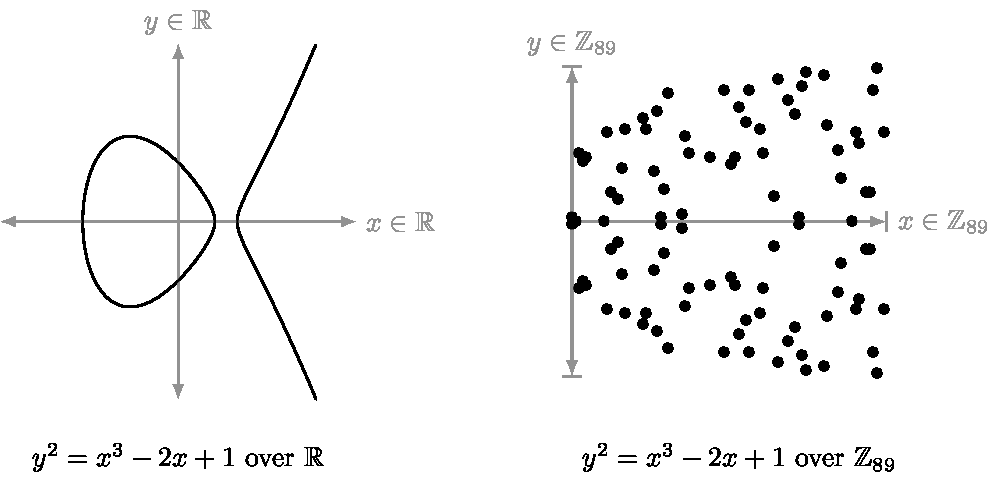
\includegraphics[width=120mm]{imagenes/curvas_Fp}
  \caption{Curva sobre $\mathbb{R}$ y sobre un cuerpo finito \cite{silverman}}
\end{figure}

Cada ecuación $y^2 = x^3 + Ax + B$ tiene asociado un discriminante $
\Delta = -16(4A^3 + 27B^2)$. Una curva es singular si y sólo si su
discriminante es $0$, en cuyo caso no sería considerada una curva
elíptica.

\begin{figure}[H] \centering
  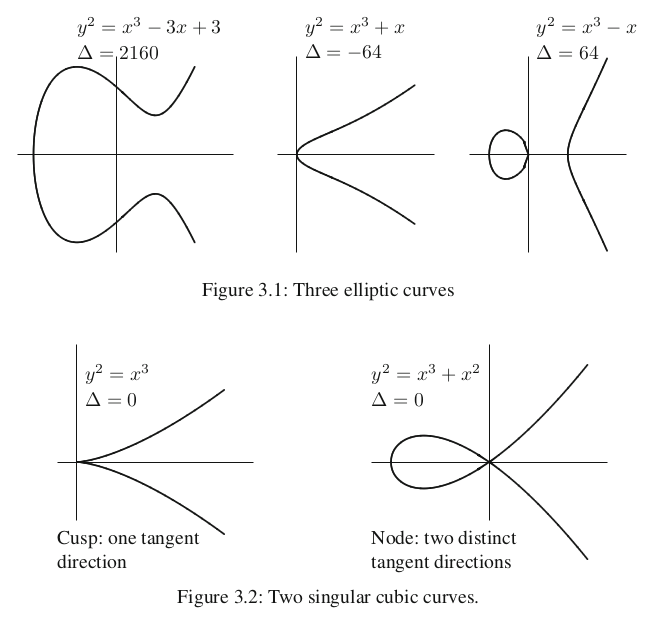
\includegraphics[width=110mm]{imagenes/curvas}
  \caption{Ejemplo de curvas elípticas \cite{silverman}}
\end{figure}

\section{Operaciones en el grupo de la curva}

En la curva elíptica podemos definir una estructura de grupo con la
operación $+$ de forma que $(E, +)$ sea un grupo abeliano. El elemento
neutro para la operación será el punto en el infinito $O$. Para
definir las operaciones en la curva vamos a recurrir a descripciones
geométricas. Estas serán fáciles de visualizar en el caso de trabajar
sobre el cuerpo de los reales, será ahí donde las ilustremos.

En primer lugar hacemos una observación: dado que la curva
$E$ es simétrica respecto del eje de abscisas podemos definir el punto
opuesto de un punto dado $P$, al que notaremos como $-P$, como el
reflejado respecto al eje de abscisas. Si $P=(x,y)$, entonces
$-P=(x,-y)$. Definimos también $-O=O$.

Consideremos dos puntos de la curva $P,Q\in E$ y la recta que las
une. Esta recta interseca a la curva $E$ en un tercer punto al que
llamamos $R$. Entonces definimos el punto $P+Q$ como el punto
reflejado respecto al eje de abcisas del punto R, es decir $-R =
P+Q$. Si $P$ y $Q$ coinciden, entonces consideramos la recta tangente
a la curva en $P$, que sería el límite de las rectas cuando $P$ y $Q$
están infinitamente cerca. Si uno de los dos puntos es $O$, trazamos
una recta vertical, consideramos el infinito “arriba”. Definimos
también $O+O=O$.

\begin{figure}[H]
  \centering
  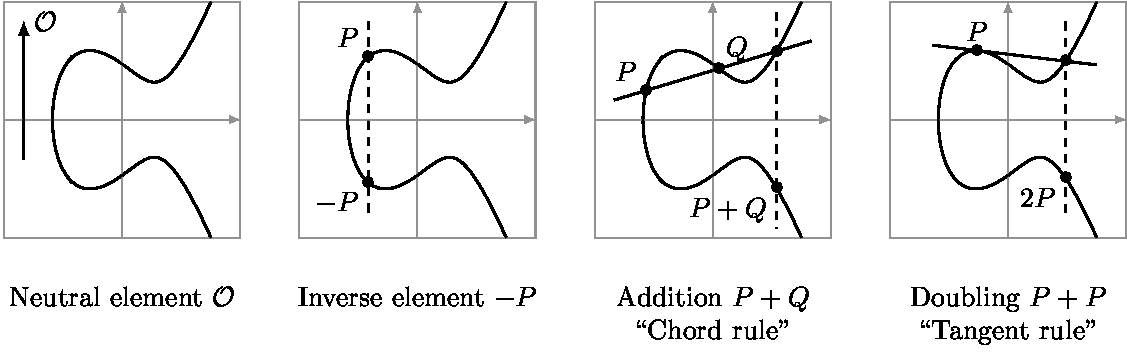
\includegraphics[width=170mm]{imagenes/operaciones}
  \caption{Estructura de grupo de curvas elípticas \cite{silverman}}
\end{figure}

Contanto las multiplicidades, la recta siempre toca a la curva en tres
puntos ($P,Q,R\in E$), y podríamos expresar esto como
$P+Q+R=O$. Examinemos los siguientes casos:

\begin{figure}[H]
  \centering
  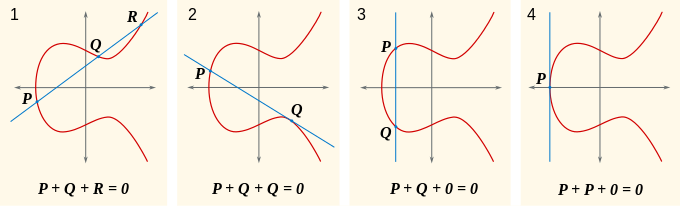
\includegraphics[width=170mm]{imagenes/suma}
  \caption{Casos de la suma en curvas elípticas. \cite{wiki:elliptic}}
\end{figure}

\begin{enumerate}
\item Los tres puntos son distintos y tenemos $P+Q=-R$.

\item El punto $Q$ tiene multiplicidad 2: además de coincidir la curva
y la recta, coinciden sus tangentes, es decir, las derivadas de ambos
polinomios en $Q$. Por lo que $R=Q$ y obtenemos $P+Q=-Q$. Este caso
también ejemplifica que $Q+Q=-P$. Este es el procedimiento cuando los
puntos coinciden.

\item $Q=-P$ y la recta es vertical. El tercer punto de corte es el
infinito, por lo que $P+Q=P+(-P)=O$. Este caso también ejemplifica que
$P+O=-(-P)=P$.

\item Tenemos $P=Q$, que tiene multiplicidad dos, y el tercer punto de
corte es el infinito. También ejemplifica que $P+O=P$.

\item Falta el caso en el que en el punto $P$ coinciden la recta con
$E$, sus tangentes, y además su curvatura, $P$ es un punto de
inflexión. Por tanto la multiplicidad de $P$ es $3$ y obtenemos
$P+P=-P$.
\end{enumerate}

\begin{figure}[H]
  \centering
  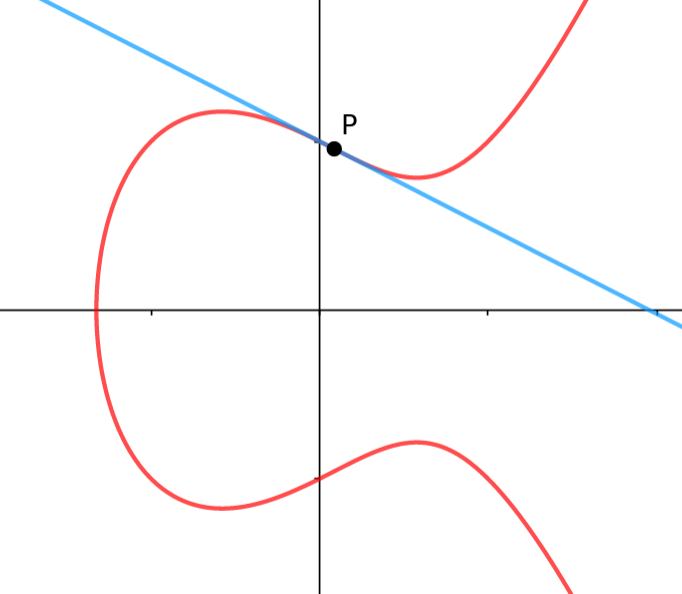
\includegraphics[width=50mm]{imagenes/suma3P}
  \caption{Caso $P+P+P = O$}
\end{figure}

Se puede comprobar que esta suma define un grupo aditivo con elemento
neutro $O$. La propiedad conmutativa es fácil de comprobar porque la
recta que une $P$ y $Q$ es la misma que la que une $Q$ y $P$, pero
demostrar la asociatividad es muy complejo.

A partir de la suma de puntos definimos el producto de un punto $P$
por un escalar $n$ como:

$$nP = \underbrace{P + P + \ldots + P}_{{n}}$$

Esta operación puede calcularse con eficiencia $O(\log n)$ escribiendo
$n$ en base $2$ y realizando duplicaciones sucesivas.

Vamos a encontrar un subgrupo cíclico $<G>\subset E(\mathbb{F}_p)$ de
una curva elíptica definida sobre un cuerpo finito
$\mathbb{F}_p$. Para ello seguimos el siguiente procedimiento:

\begin{enumerate}
\item Calculamos el número de puntos de la curva elíptica, $N =
\#E(\mathbb{F}_p)$. Esto se puede lograr mediante el
\href{https://en.wikipedia.org/wiki/Schoof%27s_algorithm}{algoritmo de
Schoof}.
\item Elegimos el factor primo mayor de $N$, al que llamaremos $n$.
\item Tomamos $h = N/n$. Para que una curva sea segura, el cofactor ha
de ser pequeño.
\item Escogemos un punto cualquiera de la curva $P\in E(\mathbb{F}_p)$
y sea $G=hP$.
\item Si $G$ es el punto en el infinito, cogemos otro punto $P$. De
esta manera, el orden de $G$ es $n$.
\end{enumerate}

Si en el paso 2, obtenemos algunos divisores de $N$ cuyo producto sea
grande, sabemos que $h$ va a ser múltiplo de ese producto y podemos
desechar la curva por insegura. Por ejemplo, si probando primos en
orden obtenemos que $11$ divide $N$, y $N/11$ no es primo, el mínimo
cofactor que podemos esperar sería $11^2$.  Este paso puede ser
computacionalmente muy costoso, pero podemos utilizar una
\href{https://safecurves.cr.yp.to/}{lista de curvas seguras} ya
conocidas con cofactor pequeño.

\section{¿Por qué las curvas elípticas son interesantes para la
criptografía?}

En 1986 fue propuesto por Koblitz y Miller un criptosistema como el de
Diffie y Hellman utilizando el grupo aditivo de las curvas elípticas
en lugar del grupo multiplicativo de los cuerpos finitos. El enunciado
del problema es el siguiente:

\textbf{Problema del logaritmo discreto:}

Sea $G$ un grupo multiplicativo y $x,y \in G$ elementos tales que $y$
está en el subgrupo generado por x, $y \in <x>$. El problema del
logaritmo discreto (DLP de sus siglas en inglés) es el problema de
determinar un entero $m\geq 1$ tal que
$$x^m=y$$

Sea $<G>$ un subgrupo aditivo de $E(K)$, el problema del logaritmo
discreto para curvas elípticas es el problema de encontrar $k$ de
manera que $kG=P$, para un punto dado $P \in <G>$.

La seguridad de las curvas elípticas en criptografía, descansa en la
dificultad de resolver este problema.

\section{Cifrado y firma con curvas elípticas}

Vamos a describir a continuación los pasos que seguirá Alice para
mandar un mensaje firmado y cifrado a Bob. Ambos se deberán poner de
acuerdo en tres parámetros, que pueden acordar por un canal de
comunicación potencialmente no seguro:

\begin{itemize}
\item Una curva $E(\mathbb{F}_p)$ segura.
\item $G$ un punto de la curva de orden primo.
\item Conocer el valor $n$ que es el orden del grupo $<G>\subset
E(\mathbb{F}_p)$.
\end{itemize}

Necesitamos que $n$ sea primo para que cualquier elemento de
$\mathbb{Z}/n\mathbb{Z}$ sea invertible.

\subsection{Claves pública y privada} Alice crea una clave privada
consistente en un entero $d_A$ elegido de manera aleatoria en el
intervalo $[1,n-1]$ y calcula un punto de la curva $Q_A=d_AG$, donde
estamos usando la multiplicación de un escalar por un punto de la
curva, que se puede realizar en tiempo $O(log d_A)$. La clave pública
de Alice será $Q_A$. Del mismo modo, la clave privada de Bob será
$d_B$ y su clave pública será $Q_B$ .

\subsection{Algoritmo de firma digital en curvas elípticas (ECDSA)}

Para firmar un mensaje, Alice sigue los siguientes pasos:

\begin{enumerate}
\item Calcula $e=HASH(m)$ el resultado de aplicar una función de
hash conocida al mensaje $m$, que lo convierte en un entero.
\item Definimos $L_n$ como el número de bits del orden del grupo,
$n$. Alice toma como $z$ el número formado por los $L_n$ bits menos
significativos de $e$.
\item-Elige de manera aleatoria un entero secreto $k$ en el
intervalo $[1,n-1]$.
\item Calcula el punto de la curva $(x_1, y_1)=kG$.
\item Toma $r = x_1 \text{ mod }n$. En el caso de que $r$ sea 0,
se vuelve al paso 3.
\item Alice calcula ahora $s=k^{-1}(z+rd_A) \text{ mod }n$. Si $s$ es 0,
se vuelve al paso 3.
\item La firma es el par $(r,s)$
\end{enumerate}

Para verificar la firma Bob necesitará conocer el mensaje y la clave
pública de Alice, el punto de la curva $Q_A$, y deberá realizar los
siguientes pasos:

En primer lugar, necesita hacer comprobaciones básicas acerca de la
información que recibe:

\begin{enumerate}
\item Comprueba que el punto $Q_A$ es un punto de la curva distinto
de $O$.
\item Se debe cumplir que $nQ_A=O$
\end{enumerate}

Si las comprobaciones anteriores son satisfactorias, Bob deberá
entonces proceder de la siguiente manera:

\begin{enumerate}
\item Comprueba que $r,s\in[1, n-1]$, en otro caso, la firma es
inválida.
\item Calcula, al igual que hacía Alice, $e$ usando la misma
función de hashing.
\item Toma de nuevo $z$ como el número formado por los $L_n$ bits menos significativos de $e$.
\item Obtiene $u_1 = zs^{-1} \text{ mod } n$ y $u_2 = rs^{-1} \text{
mod } n$.
\item Calcula el punto $C = (x_1,y_1)=u_1G+u_2Q_A$. Si $(x_1,
y_1)=O$ entonces la firma no es válida.
\item Finalmente, la firma será válida si $r= x_1 \text{ mod }
n$. En caso contrario, no lo será.
\end{enumerate}

Queda ver por qué con la operación $C=u_1G+u_2Q_A$ obtenemos el
resultado que queremos. Para ello notamos en primer lugar que
$Q_A=d_AG$ por lo que

\[ C=u_1G+u_2d_AG
\]

Ahora usamos la propiedad distributiva:

\[ C = (u_1+u_2d_A)G
\]

desarrollamos las expresiones de $u_1$ y $u_2$

\[ C = (zs^{-1}+rd_As^{-1})G
\]

y aplicamos la propiedad distributiva de nuevo con lo que

\[ C = (z+rd_A)s^{-1}G
\]

Sustituimos $s$ por su expresión tal y como se calculó en el
algoritmo:

\[ C = (z+rd_A)(z+rd_A)^{-1}(k^{-1})^{-1}G
\]

con lo que obtenemos $C = kG$

Bajo ningún concepto debemos elegir el mismo número $k$ para cifrar
dos mensajes distintos, ya que si eso ocurre podría averiguarse el
valor de $d_A$. Supongamos que tenemos dos firmas $(r, s)$, $(r,s’)$
que han sido calculadas con el mismo valor de $k$ para firmar los
mensajes $m$ y $m’$. El receptor de los mensajes podría calcular $z$ y
$z’$, dado que la función $HASH$ es pública. Puesto que $s-s’ =
k^{-1}(z-z’)$ (por el paso 6 de la creación de la firma) podría
averiguar $k = \frac{z-z’}{s-s’}$. Como $s = k^{-1}(z+d_A)$, el
receptor podría conseguir la clave privada $d_A = \frac{sk-z}{r}$.

Este fallo de implementación fue usado para extraer la clave de usada
en los sistemas PlayStation 3. También se explotaron vulnerabilidades
relacionadas con esto en la clase SecureRandom de Java para obtener
claves en aplicaciones Android que utilizaban esta implementación. Un
método para elegir valores diferentes de $k$ podría ser utilizar el
propio mensaje y la clave privada como semilla en el algoritmo
aleatorio.

\subsection{Algoritmo de cifrado en curvas elípticas}

Sea $\Phi$ una función pública invertible que transforme el mensaje un
punto de la curva $E(\mathbb{F}_p)$. Para cifrar un mensaje, Alice
sigue los siguientes pasos:

\begin{enumerate}
\item Alice elige un número $k \in [1, n-1]$.
\item El texto cifrado será $(kG, kQ_B+P_m)$, donde $P_m = \Phi(m)$.
\end{enumerate}

Para descifrarlo, Bob realiza los siguientes pasos sobre la tupla
$(C,D)$ recibida:

\begin{enumerate}
\item Bob obtiene $P_m$ así: $P_m = D - d_BC = kQ_B + P_m - d_BkG$,
puesto que $kQ_B=kd_BG=d_BkG$.
\end{enumerate}

El mensaje $m$ es $\Phi^{-1}(P_m)$.

Como $d_A Q_B=d_A d_B G=d_B d_AG=d_B Q_A$, Alice y Bob disponen de un secreto compartido que pueden utilizar para cifrado simétrico. En lugar de un número $k$, Alice puede utilizar su propia clave privada. En este caso, $C$ sería la clave pública de Alice, por lo que no es necesario transmitirla junto al mensaje (habiéndola intercambiado previamente).

\newpage

\section{RSA y ECC}

El algoritmo de RSA basa su fortaleza en el problema de la
factorización de números. Este algoritmo aparece al final de la década
de los 70. Durante los años 80, Koblitz y Miller desarrollaron la
criptografía en curvas elípticas.

Inicialmente se criticó a la criptografía de curva elípticas (ECC) por
estar basada en una matemática sobre la que no se había profundizado
de manera importante y por lo tanto podía suponer un problema de
seguridad. Se argumentaba que el problema de factorización era un
problema que se había estudiado durante siglos mientras que el
problema del logaritmo discreto era un problema que apenas tenía un
siglo de estudio.

Se usaron distintos algoritmos para intentar atacar ECC, desde los más
\textit{brutos} hasta el ataque \emph{rho de Pollard} que ya existía y
se adaptó a las curvas elípticas. Este algoritmo junto al de
\textit{baby-step/giant-step} tienen una complejidad de
$O(\sqrt{N})$. El algoritmo que hizo temer por el futuro de ECC fue
\textit{xedni} (descrito en Silverman). Se dudaba de la eficacia del
algoritmo pero los defensores del RSA, que se veían en un momento de
apogeo, vieron un punto de debilidad y quisieron proclamar que la ECC
era insegura. Se demostró que con pequeñas modificaciones este
algoritmo también se podía usar para la factorización de números y por
lo tanto ser un problema para el RSA también. Finalmente se demostró
que este algoritmo era ineficiente.

La evolución en la tecnología hizo que cada vez los números que se
usaban para el algoritmo RSA crecieran más y con ello la longitud en
bits que se necesitaba para codificarlos. Esto frente a la ECC era un
inconveniente ya que el tamaño en bits de las claves que se usaban
eran mucho menores y crecían de manera más comedida.

En esta tabla mostramos los tamaños de las claves de estos dos algoritmos, denotados $k$ y $f$, al mismo nivel de securidad.

\begin{table}[H]
\centering
\begin{tabular}{|c|c|c|}
\hline
\textbf{Security Strength} & \textbf{RSA} & \textbf{ECDSA} \\ \hline
$\leq$ 80                  & k = 1024       & f = 160 - 223  \\
112                        & k = 2048     & f = 224 - 255  \\
128                        & k = 3072     & f = 256 - 383  \\
192                        & k = 7680     & f = 384 - 511  \\
256                        & k = 15360    & f = 512+       \\ \hline
\end{tabular}
\end{table}

Finalmente, acercándonos al año 2000, la NSA sorprendió a la comunidad
anunciando su apoyo a las ECC, considerándolo un sistema seguro y
proponiendo mejoras a los algoritmos. En 2005 publicó también un
artículo en su web incitando al uso de ECC en lugar de RSA por
considerarla mucho más segura. Este hecho balancea mucho más la
discusión entre los defensores de RSA y ECC.

\section{Simulación con Openssl}

OpenSSL es una herramienta muy completa con la que hemos trabajado en la
asignatura y que además nos da la facilidad para trabajar también con curvas
elípticas. En esta práctica vamos a realizar pasos análogos a lo que hemos visto
durante el curso pero aplicando la teoría de curvas elípticas. 

Durante nuestros intentos de cifrar y descifrar utilizando ECC hemos encontrado
\href{https://stackoverflow.com/a/58942471/2588566}{este comentario} donde se
nos indica que no podemos realizar estos pasos directamente usando ECC. Usamos
lo que se ha llama \textit{Elliptic Curve Integrated Encryption Scheme}.

\subsection{Taller de criptografía}

En primer lugar comentamos que OpenSSL nos ofrece una serie de curvas ya
definidas en su utilidad para terminal. Tenemos la posibilidad de listar las
curvas disponibles utilizando:

\begin{lstlisting}[language=bash]
  openssl ecparam -list_curves
\end{lstlisting}

tras ejecutar esta instrucción se nos mostrará una lista con distintas curvas
conocidas. Para continuar con el taller vamos a elegir una de estas curvas,
en nuestro caso \textit{secp256k1} que es una curva famosa y bastante segura.

Para crear un archivo de configuración para la curva utilizamos 

\begin{lstlisting}[language=bash]
  openssl ecparam -name secp256k1 -out secp256k1.pem
\end{lstlisting}

que creará un achivo \textit{secp256k1.pem} con información sobre la curva. Si
ahora hacemos

\begin{lstlisting}[language=bash]
  openssl ecparam -in secp256k1.pem -text -param_enc explicit -noout
\end{lstlisting}

obtenemos información sobre los parametros elegidos como: 

\begin{itemize}
  \item Los parámetros $A$ y $B$ de la ecuación de la curva.
  \item El número primo elegido para el cuerpo sobre el que se construye la curva.
  \item El generador del punto cíclico, $G$.
  \item El orden del grupo $<G>$.
  \item El cofactor del grupo cíclico.
\end{itemize}

Una vez elegida la curva procedemos ahora a crear la clave privada. Para ello
utilizamos 

\label{genkey}
\begin{lstlisting}[language=bash]
  openssl ecparam -in secp256k1.pem -genkey -noout -out userS-privkey.pem
\end{lstlisting}

Con esta orden le indicamos que genere en un archivo \textit{userS-privkey.pem}
una clave privada partiendo del archivo de configuración para la curva que hemos
generado anteriormente. Si deseamos ver la información de la clave privada y la pública asociada que
hemos generado podemos usar 

\begin{lstlisting}[language=bash]
  openssl ec -in userS-privkey.pem -text -noout
\end{lstlisting}

Si queremos guardar la clave pública en un archivo tenemos que hacer 

\begin{lstlisting}[language=bash]
  openssl ec -in userS-privkey.pem -pubout -out userS-pubkey.pem
\end{lstlisting}

donde a partir de nuestra clave privada generamos un archivo de clave pública
con la clave pública generada. Para ver la información almacenada en el nuevo
archivo ejecutamos

\begin{lstlisting}[language=bash]
  openssl ec -in userS-pubkey.pem -pubin -text -noout
\end{lstlisting}

En este paso podemos comprobar  que el contenido coincide con la información que
obtuvimos al generar la clave privada.

Procedemos a firmar ahora un mensaje. Creamos un archivo para ello que hemos
llamado \textit{msg.txt} y procedemos a firmarlo utilizando la clave privada que
hemos generado con anterioridad.

\begin{lstlisting}[language=bash]
  openssl dgst -sign userS-privkey.pem -out msg.txt.sign msg.txt
\end{lstlisting}

Para realizar el cifrado creamos un secreto compartido generado a partir de nuestra clave
privada y la clave pública del receptor (suponiendo las claves generadas e intercambiadas). Esto lo hacemos por que OpenSSL no nos permite cifrar directamente
usando el archivo de la clave privada generada en los primeros pasos.

\begin{lstlisting}[language=bash]
  openssl pkeyutl -derive -inkey userS-privkey.pem \
    -peerkey userR-pubkey.pem -out secret.txt
\end{lstlisting}

Ciframos ahora utilizando el archivo \textit{secreto.txt} generado como clave

\begin{lstlisting}[language=bash]
  openssl enc -aes-256-cbc -md sha512 -pbkdf2 -iter 100000 -salt \
   -in msg.txt -out msg.txt.enc -pass file:secret.txt
\end{lstlisting}

además le hemos indicado que usamos \textit{sha512} como función de resumen y
\textit{aes-256-cbc} como sistema de cifrado.

Ahora el receptor del mensaje debe seguir los siguientes pasos. En
primer lugar crea el mismo secreto, pero esta vez usando su clave privada y la clave pública del emisor

\begin{lstlisting}[language=bash]
  openssl pkeyutl -derive -inkey userR-privkey.pem -peerkey \
    userS-pubkey.pem -out secret.txt
\end{lstlisting}

Para descrifrar se añade la opción \texttt{-d}

\begin{lstlisting}[language=bash]
  openssl enc -aes-256-cbc -md sha512 -pbkdf2 -iter 100000 -salt -d \
    -in msg.txt.enc -out msg.txt -pass file:secret.txt
\end{lstlisting}

Y por último para verificar la firma del documento usamos la clave pública del emisor y el documento de la firma sobre el documento que hemos
obtenido al descifrar.

\begin{lstlisting}[language=bash]
  openssl dgst -verify userS-pubkey.pem -signature msg.txt.sign msg.txt
\end{lstlisting}

\nocite{*}
\addcontentsline{toc}{section}{Referencias}
\bibliographystyle{unsrt}
\bibliography{example}

\end{document}
